%% PCN chip paper — ArXiv preprint v3rev
%% Target: cs.AR + cs.NE cross-listing
%% v3: restructured and tightened from v2; unified comparison sections,
%%     compressed peripherals, fixed 5nm/7nm inconsistency, sharper argument thread
%% v3rev: email updated; GitHub URL added; Claude Code acknowledgement; MNIST/EMNIST note
%%
\documentclass[journal,10pt,twoside]{IEEEtran}

\usepackage{cite}
\usepackage{amsmath,amssymb,amsfonts}
\usepackage{graphicx}
\usepackage{booktabs}
\usepackage{array}
\usepackage{xcolor}
\usepackage{hyperref}
\usepackage{siunitx}
\usepackage{subcaption}
\usepackage{bm}

%% Raggedright paragraph column type (avoids justification artefacts in narrow p{} cols)
\newcolumntype{P}[1]{>{\raggedright\arraybackslash}p{#1}}

\begin{document}

\title{Scalable Modular Analog VLSI for Predictive Coding Networks:\\
       Temporal Multiplexing, Learned Routing, and Zero Weight Bandwidth}

\author{Saul Dobney%
  \thanks{Correspondence: saul.dobney@dobney.com.
  Design files, RTL, and simulation scripts are available at
  \url{https://github.com/dobneyresearch/PredictiveCodingNetworks_AnalogVLSIdesign}.}%
}

\maketitle

%% ─────────────────────────────────────────────────────────────────────────────
\begin{abstract}
We present the first analog CMOS implementation of a Predictive Coding
Network (PCN) with unsupervised on-chip Hebbian learning, verified in the
open-source SkyWater 130\,nm process (Sky130A).
A concurrent digital RTL implementation~\cite{oh2026synthesizable} executes
supervised predictive-coding dynamics in synthesizable hardware; the present
work addresses a complementary design space: analog weight storage,
unsupervised Hebbian learning, and zero off-chip weight bandwidth.
The design eliminates the memory bandwidth bottleneck that limits digital
neural inference: weights are stored as voltages on 200\,fF capacitors
within a five-transistor OTA, computed by transconductance, and accumulated
by Kirchhoff's current law — no weight data crosses the chip boundary
during inference.

Three structural contributions address the principal limitations of prior
analog neuromorphic hardware:

\textbf{(1) Temporal layer reuse.}
A single 16$\times$16 physical MAC array is multiplexed across $N_\text{virt}$
virtual network layers via an 8-bit ADC activation save-and-reload cycle
orchestrated by a 22-state FSM, decoupling network depth from silicon area.
The ADC--DAC reload resets the differential-pair common mode at each virtual
layer, providing consistent 6.68\,V/V module gain independent of cascade
depth — a property the spatial cascade does not have.
Module-level gains across the four physical layers are verified in SPICE:
1.43, 0.45, 0.70, and 0.54\,V/V in the untrained state,
self-corrected by Hebbian adaptation.

\textbf{(2) Dynamic inter-layer routing.}
Inter-module prediction connections are themselves capacitive weight cells
updated by the same Hebbian rule as MAC weights, but at a slower timescale
set by a larger routing capacitor ($C_{w,\text{route}} = 2$\,pF).
The routing Hebbian LTD write mechanism is verified in Sky130A SPICE
($\Delta V_{w,\text{route}} \approx -45$\,mV/pulse, self-correcting error
flag confirmed), allowing the network topology to adapt from data rather
than being fixed at tape-out.

\textbf{(3) A complete, open-source, simulation-verified proof-of-concept.}
The digital controller (1,117 standard cells; place-and-route closed at
$+8.46$\,ns setup margin with zero routing DRC violations on Sky130A)
and all analog blocks are SPICE-verified.
A hardware-calibrated Python/NumPy simulation demonstrates 484$\times$
single-step prediction error reduction and 483$\times$ specificity on a
synthetic template task, and identifies GHA with sequential deflation as
the correct training rule for this architecture.
All design files, RTL, and simulation scripts target the Efabless OpenMPW
shuttle for fabrication.
\end{abstract}

\begin{IEEEkeywords}
analog neuromorphic computing, predictive coding, Hebbian learning,
temporal multiplexing, dynamic routing, current-mode circuits,
scalable architecture, Sky130, OpenMPW
\end{IEEEkeywords}

%% ─────────────────────────────────────────────────────────────────────────────
\section{Introduction}
\label{sec:intro}

The dominant cost of running a neural network on modern hardware is not
arithmetic — it is memory.
An NVIDIA H100 GPU delivers 2{,}000\,TOPS (INT8) at 700\,W,
but when running large-model inference its arithmetic units are idle
for more than 90\% of cycles while waiting for weights to arrive from
high-bandwidth memory (HBM) at 3.35\,TB/s~\cite{nvidia2022h100}.
For a 7-billion-parameter model, each forward pass requires reading 14\,GB
of weight data; at 3.35\,TB/s, this bounds throughput regardless of
compute capacity.
The memory bandwidth wall is the defining limitation of digital neural
inference at scale.

The brain avoids this wall by a simple principle: \emph{compute where data
lives}.
Each synapse holds its own weight, computes its own product, and contributes
its result via a shared wire — no weight fetch, no bus, no serialisation.
Predictive Coding Networks~(PCNs)~\cite{rao1999predictive} formalise this
algorithmically: learning proceeds by minimising local prediction errors
via a Hebbian rule that depends only on the local error signal and
pre-synaptic activation, requiring no global
backpropagation~\cite{bogacz2017tutorial}.
This \emph{locality} property maps cleanly to analog VLSI:
the weight is the capacitor voltage, the multiply is the transistor
transconductance, and the accumulate is Kirchhoff's current law on a shared
wire~\cite{mead1989analog}.

Despite these advantages, practical analog learning hardware has faced
three structural barriers:

\textbf{Barrier~1 — Weight density.}
A conventional analog MAC array requires one physical synapse per weight.
At 60--100\,\textmu m$^2$/cell in 130\,nm CMOS,
a single 16$\times$16 array holds only 256 weights — insufficient for
any meaningful task.

\textbf{Barrier~2 — Fixed topology.}
Inter-layer connectivity is determined at tape-out.
The network can strengthen or weaken existing connections but cannot
discover which source features predict which destination features,
nor adapt to changing input statistics.

\textbf{Barrier~3 — Analog power.}
Quiescent tail current through MAC cells dominates power consumption.
Without deliberate co-scaling of the precision gate and tail current,
the array draws power proportional to cell count regardless of activity.

This paper addresses all three barriers with a complete, simulation-verified
proof-of-concept.
Our contributions are:

\textbf{(1) Temporal layer reuse} (Section~\ref{sec:temporal}).
A single MAC array is multiplexed across $N_\text{virt}$ virtual layers via
ADC activation save-and-reload, multiplying effective weight capacity by
$N_\text{virt}$ with no additional analog area and providing a guaranteed
common-mode reset at each virtual layer.

\textbf{(2) Learned inter-layer routing} (Section~\ref{sec:routing}).
Inter-module prediction connections are themselves Hebbian weight cells at
a slower timescale, allowing the network topology to self-organise from
data with no additional learning hardware.

\textbf{(3) Power co-scaling analysis} (Section~\ref{sec:power}).
We derive the precision-gate co-scaling constraint that governs the achievable
power floor and project a $10{,}000\times$ pathway from the 80\,mW baseline
to an $\approx$8.5\,mW operating point.

\textbf{(4) Validated open-source implementation} (Sections~\ref{sec:physical}
and~\ref{sec:results}).
SPICE-verified analog blocks, synthesised Verilog RTL, a place-and-routed
GDS, and a hardware-calibrated algorithmic simulation demonstrate end-to-end
correctness and identify the correct training rule from simulation failures.

Section~\ref{sec:background} reviews PCN theory and prior hardware.
Sections~\ref{sec:architecture}--\ref{sec:digital} describe the system,
cell, temporal reuse, routing, and digital controller.
Section~\ref{sec:physical} reports physical implementation results.
Sections~\ref{sec:power}--\ref{sec:scalability} analyse power and
scalability.
Section~\ref{sec:results} presents algorithmic validation.
Section~\ref{sec:discussion} discusses limitations and future directions.

%% ─────────────────────────────────────────────────────────────────────────────
\section{Background}
\label{sec:background}

\subsection{Predictive Coding Networks}

A PCN is a hierarchical model with $L$ layers, each maintaining a
representation $\mathbf{r}^{(\ell)}$ and weight matrix $\mathbf{W}^{(\ell)}$.
Layer $\ell$ generates the top-down prediction
$\hat{\mathbf{r}}^{(\ell-1)} = f(\mathbf{W}^{(\ell)\top}\mathbf{r}^{(\ell)})$
and computes the local prediction error:
\begin{equation}
\boldsymbol{\varepsilon}^{(\ell)} =
  \mathbf{r}^{(\ell)} - f(\mathbf{W}^{(\ell+1)\top}\mathbf{r}^{(\ell+1)}).
\label{eq:pcn_error}
\end{equation}
Weights undergo the local Hebbian update:
\begin{equation}
\Delta\mathbf{W}^{(\ell)} \propto
  \boldsymbol{\varepsilon}^{(\ell-1)}\,{\mathbf{r}^{(\ell)}}^\top,
\label{eq:pcn_hebb}
\end{equation}
which depends only on signals physically present at the synapse.
Under appropriate conditions this is equivalent to
expectation-maximisation on a Gaussian generative
model~\cite{bogacz2017tutorial}.

Sanger's Generalised Hebbian Algorithm~(GHA)~\cite{Sanger1989} extends
Oja's rule with sequential deflation,
$\mathbf{x}^{(i+1)} = \mathbf{x}^{(i)} - (\mathbf{w}_i^\top\mathbf{x})\mathbf{w}_i$,
guaranteeing convergence of the row span to the top-$N_H$ principal subspace.
Section~\ref{sec:results} identifies GHA as the correct training rule for
this architecture and explains why simpler variants fail.

\subsection{Prior Analog Neuromorphic Hardware}

Analog computation for neural inference is well
established~\cite{shibata1992neuron}.
Floating-gate synapses~\cite{diorio1996single} provide compact non-volatile
weight storage but require UV erasure or specialised charge-pump circuits.
Phase-change memory~\cite{ambrogio2018equivalent} and resistive
RAM~\cite{prezioso2015training} offer multi-level non-volatile storage at
the cost of back-end process integration.
Digital neuromorphic processors (Loihi~2~\cite{davies2018loihi},
BrainScaleS-2~\cite{pfeiffer2018deep}) implement spike-based learning.
To our knowledge, no prior work has implemented a rate-coded PCN with
continuous on-chip Hebbian learning in standard CMOS,
with verified multi-chip scaling and dynamic topology adaptation.

%% ─────────────────────────────────────────────────────────────────────────────
\section{System Architecture}
\label{sec:architecture}

\subsection{Modular Hierarchy}

The PCN design is organised in four levels:

\textbf{MAC array.}
$N_\text{rows} \times N_\text{cols}$ analog weight cells with $N_\text{rows}$
KCL accumulation buses.
All rows compute simultaneously; one forward pass completes in
$\tau_\text{KCL} = R_\text{err} \times C_\text{KCL} \approx 28\,\text{ns}$.
KCL bandwidth ($f_\text{KCL} \approx 5.7\,\text{MHz}$) is invariant to
array size by scaling $R_\text{err} \propto 1/N_\text{cols}$
(Section~\ref{sec:power}).

\textbf{Tile.}
A stack of $D$ MAC arrays connected by layer-link circuits providing
ascending source-follower (data upward) and descending prediction current
(top-down).
In temporal reuse mode the tile degenerates to a single array cycling
through $N_\text{virt}$ virtual layers.

\textbf{Chip.}
Multiple tiles on one die, each independently biased and controlled.
Adding tiles increases weight capacity and throughput linearly with no
electrical coupling between tiles.

\textbf{System.}
The activation save/reload cycle produces 8-bit digital activation pages
transmitted over SPI between chips.
No inter-chip analog signal path is required.
Adding a chip adds weight capacity and throughput simultaneously with no
shared-memory bottleneck.

\subsection{Chip Summary}

Tables~\ref{tab:chip_summary} and~\ref{tab:chip_area} specify the Sky130A
proof-of-concept, targeting Efabless Caravel as a Wishbone-peripheral user
project.
The chip implements a four-layer PCN: four $16{\times}16$ MAC arrays
stacked vertically and connected pairwise by three \texttt{layer\_link}
circuits.
The full stack contains $4 \times 256 = 1{,}024$ physical MAC cells and
1,024 independently learned weights in $\approx$0.33\,mm$^2$ of analog area.
No weight data crosses the chip boundary during inference.

\begin{table}[t]
\caption{Sky130A proof-of-concept: architecture and compute parameters}
\label{tab:chip_summary}
\centering
\footnotesize
\begin{tabular}{@{} l l >{\raggedright\arraybackslash}p{2.1cm} @{}}
\toprule
Parameter & Value & Notes \\
\midrule
\multicolumn{3}{@{}l}{\textit{Process and supply}} \\
Process node & Sky130A & SkyWater 130\,nm \\
Supply voltage & 1.8\,V & \\[3pt]
\multicolumn{3}{@{}l}{\textit{Physical stack}} \\
PCN layers & 4 & spatial stack \\
Array per layer & $16{\times}16$ & 256 MAC cells \\
Total MAC cells & 1,024 & $4{\times}256$ \\
Physical weights & 1,024 & one per cell \\
KCL settling time & 28\,ns & $R_\text{err}{\times}C_\text{KCL}$ \\
Throughput (4-layer) & 5.9\,GOPS & continuous \\[3pt]
\multicolumn{3}{@{}l}{\textit{Temporal reuse}} \\
Weight pages (SRAM) & 4 & 1\,kB $\div$ 256\,B/page \\
Effective weights (N=4) & 4,096 & $1{,}024{\times}4$ pages \\
Effective weights (N=100) & 102,400 & requires 100\,kB SRAM \\[3pt]
\multicolumn{3}{@{}l}{\textit{Weight cell}} \\
Topology & 5T OTA & MN1/2, MP1/2, MN3 \\
Weight capacitor $C_w$ & 200\,fF & NFET gate cap \\
CMOS TG & MN4+MP4 & write access \\
$V_w$ range & 0.50--1.35\,V & codes 71--192 \\
Weight resolution & ${\approx}$6.6\,bits & 114 usable codes \\
Hebbian step & ${\approx}$5\,mV/pulse & hardware-verified \\[3pt]
\multicolumn{3}{@{}l}{\textit{Digital controller}} \\
Clock & 50\,MHz & \\
Standard cells & 1,117 & Sky130 HD \\
SRAM & 1\,kbyte & OpenRAM \\
Setup WNS & $+$8.46\,ns & TT corner \\
\bottomrule
\end{tabular}
\end{table}

\begin{table}[t]
\caption{Sky130A proof-of-concept: silicon area and power}
\label{tab:chip_area}
\centering
\footnotesize
\begin{tabular}{@{} l l >{\raggedright\arraybackslash}p{2.0cm} @{}}
\toprule
Parameter & Value & Notes \\
\midrule
\multicolumn{3}{@{}l}{\textit{Silicon area}} \\
MAC cell (target) & ${\approx}600$\,\textmu m$^2$ & $10{\times}8$\,\textmu m \\
4-layer analog stack & ${\approx}330{,}000$\,\textmu m$^2$ & 0.33\,mm$^2$ \\
Digital + SRAM (P\&R) & ${\approx}570{,}000$\,\textmu m$^2$ & 0.57\,mm$^2$ \\
\textbf{Total die (estimate)} & ${\approx}$\textbf{0.90\,mm}$^2$ & \\[3pt]
\multicolumn{3}{@{}l}{\textit{Power (4-layer chip, baseline)}} \\
One MAC layer & 18.9\,mW & $256{\times}I_\text{tail}{\times}V_\text{DD}$ \\
4-layer chip & ${\approx}80$\,mW & incl.\ layer-links \\
With duty cycle + gating & ${\approx}0.8$\,mW & 10\% duty, 50\% rows \\
Digital only & ${\approx}36$\,\textmu W & \\
Off-chip weight bandwidth & 0 & voltages on $C_w$ \\[3pt]
\multicolumn{3}{@{}l}{\textit{Effective capacity (full 10\,mm$^2$ die, Sky130A)}} \\
Physical cells & ${\approx}16{,}000$ & at 600\,\textmu m$^2$/cell \\
With $N_\text{virt}{=}100$ & ${\approx}1.6$\,M & effective weights \\
\bottomrule
\end{tabular}
\end{table}

%% ─────────────────────────────────────────────────────────────────────────────
\section{MAC Cell Design}
\label{sec:mac}

\subsection{Topology}

The MAC cell is a five-transistor PMOS-load OTA with a capacitive weight
store.
MN1 and MN2 form a differential pair; their shared tail current is set by
the gate voltage of MN3.
MP1 and MP2 form a 1:1 PMOS current mirror that converts differential drain
current to a single-ended output $I_\text{out}$ at the drain of MP2,
accumulating onto the row-shared KCL bus to compute
$\mathbf{y} = \mathbf{W}\mathbf{x}$ in the current domain.

The weight is stored as voltage $V_w$ on $C_w$.
$V_w$ drives MN3's gate directly, so
$I_\text{tail} \propto (V_w - V_\text{th,N})^2$,
giving a quadratic weight-to-current mapping absorbed by calibration in
the weight DAC encoding.
Single-cell gain at mid-scale ($V_w = 0.9\,\text{V}$) with
$R_L = 100\,\text{k}\Omega$ is 6.82\,V/V in SPICE (Sky130A, TT, 27$^\circ$C).

The coupling of $V_w$ to $I_\text{tail}$ means $V_\text{iout}$ varies with
$V_w$; upper physical layers in a spatial stack experience elevated
common-mode after the PMOS source-follower level-shift, reducing module
gain to 0.45--0.70\,V/V at layers~1--3 in the untrained state.
Hebbian learning self-calibrates by raising $V_w$ in upper layers as it
minimises prediction error.
Temporal reuse (Section~\ref{sec:temporal}) eliminates this calibration
requirement entirely by resetting $V_\text{cm}$ at each virtual layer.
A Gilbert-cell topology~\cite{gilbert1968precise} with independent tail
biasing would remove the $V_w$--operating-point coupling structurally.

\subsection{Weight Storage and CMOS Transmission Gate}

$C_w$ is charged by write current $I_\text{write}$ through a CMOS
transmission gate (TG) formed by NMOS MN4 ($W/L = 0.5/0.5\,\mu\text{m}$)
and PMOS MP4 ($W/L = 1.0/0.35\,\mu\text{m}$) in parallel.
The complementary PMOS path extends the usable $V_w$ range to
$0.50\text{--}1.35\,\text{V}$ ($\approx$6.6 effective bits, codes 71--192).

Gate-induced drain leakage from MP4 causes $V_w$ to drift upward at
$\approx$20\,mV/ms during hold — negligible relative to the Hebbian update
step ($\approx$5\,mV per pulse).
During idle periods the SRAM shadow stores the digital weight word;
the controller refreshes $V_w$ on wake-up.
Weight persistence is verified in SPICE through the full chain
SRAM $\to$ 8-bit R-2R DAC $\to$ TG $\to$ $C_w$,
with write errors $<1.5$\,LSB across the full range.

\subsection{Simulation Characterisation}

Table~\ref{tab:mac_char} summarises SPICE-measured MAC cell parameters.

\begin{table}[t]
\caption{MAC cell SPICE characterisation (Sky130A, TT, 27\,$^{\circ}$C)}
\label{tab:mac_char}
\centering
\small
\begin{tabular}{P{2.3cm}rP{2.9cm}}
\toprule
Parameter & Value & Condition \\
\midrule
Single-cell gain $A_v$ & 6.82\,V/V & $V_w = 0.9\,\text{V}$, $R_L=100\,\text{k}\Omega$ \\
Spatial mod0 gain & 1.43\,V/V & $V_w=0.75\,\text{V}$; 4-layer testbench \\
Spatial mod1--3 gain & 0.45--0.70\,V/V & untrained; Hebbian self-calibrates \\
Temporal gain & 6.68\,V/V & $N_\text{virt}=1$, reset to $V_\text{cm}$ \\
Tail current $I_\text{tail}$ & $\approx$230\,\textmu A & $V_w = 0.90\,\text{V}$ \\
Tail current (low power) & $\approx$1\,\textmu A & $V_w = 0.53\,\text{V}$ \\
$V_w$ range (CMOS TG) & 0.50--1.35\,V & codes 71--192 \\
SAR ADC latency & 10 cycles & BITS+2 \\
Weight write error & $<$1.5\,LSB & across full range \\
Hebbian $\Delta V_w$ & $\approx$5\,mV/pulse & at operating point \\
Routing $\Delta V_{w,\text{route}}$ & $\approx -45$\,mV/pulse & LTD, routing testbench \\
\bottomrule
\end{tabular}
\end{table}

%% ─────────────────────────────────────────────────────────────────────────────
\section{Temporal Layer Reuse}
\label{sec:temporal}

\subsection{The Spatial Cascade and PMOS Source-Follower Level Shift}
\label{sec:spatial}

In a spatial multi-layer stack, the balanced output voltage of a
$16{\times}16$ module is $V_\text{iout,bal} = 0.468\,\text{V}$, set by
equilibrium between the current-subtractor's diode-connected PMOS load and
the CLM-induced current imbalance.
This lies below the NMOS threshold ($V_\text{th,N} \approx 0.48\,\text{V}$);
a naive NMOS source follower would collapse the upper layer's gain.

The layer link therefore uses a \textbf{PMOS source follower}, which
\emph{raises} the signal by $|V_{gs,P}| \approx +0.67\,\text{V}$,
giving $V_\text{inp}^{(1)} = 0.468 + 0.67 = 1.137\,\text{V}$.
A matched reference PMOS SF biased at $V_\text{cm,iout} = 0.468\,\text{V}$
generates $V_\text{cm,upper} = 1.137\,\text{V}$, preserving the
differential signal:
\begin{equation}
  V_\text{inp,upper} - V_\text{cm,upper} = V_\text{iout,lower} - V_\text{cm,iout}.
\end{equation}

The full 4-layer $16{\times}16$ cascade is verified in ngspice
(Sky130A, TT, 27$^\circ$C) with a $\pm50\,\text{mV}$ DC sweep:
mod0 $= 1.43$, link01 SF $= 0.79$, mod1 $= 0.45$, link12 SF $= 0.81$,
mod2 $= 0.70$, link23 SF $= 0.81$, mod3 $= 0.54\,\text{V/V}$.
Signal propagates through all four physical layers.
The gain reduction at layers~1--3 reflects the untrained operating point;
Hebbian learning raises $V_w$ to restore tail current and module gain
as it minimises prediction error.

\subsection{Temporal Reuse Architecture}

Each temporal inference cycle proceeds in four phases:

\textbf{Phase~1 — Activation save.}
All $N_\text{cols}$ column outputs are digitised by the 8-bit SAR ADC
(10 clock cycles per column) and written to the activation SRAM.

\textbf{Phase~2 — Weight reload.}
The SRAM weight page for the next virtual layer is read; the weight DAC
drives $V_w[r,c]$ for each cell.

\textbf{Phase~3 — Activation replay.}
The activation SRAM is read back; the 8-bit R-2R input DAC drives
$V_\text{inp}[c]$ relative to $V_\text{cm}$, resetting the differential
pair's common mode regardless of the previous layer's output.
SPICE simulation confirms $V_\text{inp,cm}$ stays within
$\pm 25\,\text{mV}$ of $V_\text{cm} = 0.9\,\text{V}$ across all four
virtual layers — the operating-point reset the source follower cannot provide.

\textbf{Phase~4 — Compute.}
With activations stable and weights loaded, the array computes
$\mathbf{y}_\text{virt} = \mathbf{W}_\text{virt}\mathbf{x}_\text{virt}$
via KCL.
The precision gate determines whether Hebbian updates are applied.

The GHA training rule (Section~\ref{sec:results}) is implemented in firmware:
for row $i$, the controller loads the deflated residual
$\mathbf{x}^{(i)} = \mathbf{x} - \sum_{k<i}(\mathbf{w}_k^\top\mathbf{x})\mathbf{w}_k$
via \texttt{INP\_DAC\_DATA} (register~0x2C), triggers a standalone ADC sweep
via \texttt{CTRL[6]}, and gates Hebbian pulses to row $i$ only via
\texttt{HEBB\_ROW\_MASK} — requiring no additional analog hardware.

\subsection{Effective Weight Density}

\begin{table}[t]
\caption{Effective weight density: spatial vs.\ temporal reuse.
Production projections carry the same architecture to commercial nodes.}
\label{tab:density}
\centering
\small
\begin{tabular}{P{3.0cm}rrr}
\toprule
Configuration & Phys.~cells & $N_\text{virt}$ & Eff.~wts \\
\midrule
Spatial (na\"{i}ve) & 256 & 1 & 256 \\
Temporal $N=8$ & 256 & 8 & 2,048 \\
Temporal $N=100$ & 256 & 100 & 25,600 \\
\midrule
\multicolumn{4}{l}{\emph{Production projections (same architecture)}} \\
Sky130, $N=100$, $32\times64$ arr. & 2,048 & 100 & 204,800 \\
28\,nm, $N=100$ & $\sim$16{,}000 & 100 & $\sim$1.6\,M \\
7\,nm, $N=100$, 10\,mm$^2$ die & $\sim$1{,}000{,}000 & 100 & $\sim$100\,M \\
\bottomrule
\end{tabular}
\end{table}

Table~\ref{tab:density} shows effective weight counts.
The primary advantage of temporal reuse over the spatial cascade is
operating-point consistency: the ADC--DAC reload resets $V_\text{inp,cm}$
precisely to $V_\text{cm}$ at each virtual layer, giving consistent
6.68\,V/V module gain regardless of cascade depth (Section~\ref{sec:circuit}).

%% ─────────────────────────────────────────────────────────────────────────────
\section{Dynamic Inter-Layer Routing}
\label{sec:routing}

\subsection{Motivation: Fixed Topology as a Learning Constraint}

In the current design, inter-module prediction connectivity is fixed at
tape-out.
The Hebbian rule can adjust weight magnitudes within a fixed topology but
cannot discover which source features are statistically predictive of which
destination features, create skip connections, or bypass redundant rows.

\subsection{Routing Weights}

Inter-module prediction connectivity is structurally identical to synaptic
weight at a higher hierarchical level.
A routing weight $V_{w,\text{route}}[r_\text{dest}, j]$ modulates how
strongly source row $j$'s prediction current contributes to destination
row $r_\text{dest}$:
\begin{equation}
I_\text{pred}[r_\text{dest}] = \sum_j\,
  f\!\left(V_{w,\text{route}}[r_\text{dest},j]\right) \cdot
  g\!\left(V_\text{iout}^\text{upper}[j]\right),
\label{eq:routing}
\end{equation}
stored on the same 200\,fF capacitor as a MAC weight and updated by the
same Hebbian current pulse.
The update condition,
$\Delta V_{w,\text{route}}[r_\text{dest}, j] \propto
  \text{activity}(\text{source}_j) \times \varepsilon[r_\text{dest}]$,
strengthens a routing connection whenever source row $j$ is active and
destination row $r_\text{dest}$ has a non-zero prediction error — exactly
the condition under which that connection is useful.

\subsection{Two-Timescale Adaptation}

Routing weights use a larger storage capacitor
($C_{w,\text{route}} = 2\,\text{pF}$, $10\times C_w$), giving
$\Delta V_{w,\text{route}} \approx 0.5\,\text{mV/pulse}$ — a $10\times$
slower topological timescale requiring no additional hardware.
Fast timescale (MAC weights): synaptic strengths adapt within the current
routing skeleton.
Slow timescale (routing weights): the skeleton rewires toward statistical
dependencies in the input, mirroring the developmental sequence of rapid
synaptic potentiation followed by slower structural pruning in biological
cortex.

A parameter-efficient variant uses a $K$-dimensional routing score,
$R[r_\text{dest},j] = \sigma(\mathbf{p}_{r_\text{dest}}^\top\,\mathbf{id}_j)$,
analogous to the query-key dot product in transformer
attention~\cite{vaswani2017attention} but computed in the analog domain
by the same OTA array and updated by the same Hebbian rule.

\subsection{Sky130A Verification}

The routing Hebbian write mechanism was verified in a 16$\times$32 testbench.
Source row~0 active ($+200\,\text{mV}$); error flag ierr\_dig = HIGH.
After 7 LTD pulses:
$V_{w,\text{route}}$ decreased from 0.750\,V to 0.596\,V
($\Delta V = -45\,\text{mV/pulse}$, confirmed LTD).
By $t = 380\,\text{ns}$, ierr\_dig fell from 1.8\,V to 0.12\,V,
demonstrating the self-correcting error loop.
End-to-end convergence of routing weights to a learned topology
is a direction for future experimental work.

%% ─────────────────────────────────────────────────────────────────────────────
\section{Analog Peripherals and Digital Controller}
\label{sec:peripherals}

\subsection{Analog Peripherals}

Table~\ref{tab:peripherals} summarises the analog peripheral circuit
specifications, all SPICE-verified (Sky130A, TT, 27$^\circ$C).

\begin{table}[t]
\caption{Analog peripheral circuits: specifications and verification
(Sky130A, TT, 27$^\circ$C)}
\label{tab:peripherals}
\centering
\footnotesize
\begin{tabular}{P{1.9cm}P{2.3cm}P{3.1cm}}
\toprule
Block & Key parameter & Verified value \\
\midrule
Bias generator & $V_\text{bias,n}$ / $V_\text{cm}$ / $V_\pi$ & 0.760 / 0.900 / 0.650\,V ($<$1\,mV error) \\
PMOS SF (layer link) & Level shift & $+0.67$\,V; $V_\text{inp}^{(1)} = 1.137$\,V \\
Pred. divider (layer link) & $R_1{=}300\,\text{k}\Omega$, $R_2{=}500\,\text{k}\Omega$ & descending prediction path \\
Weight DAC (8-bit R-2R) & DNL at code 128 & $<$0.06\,LSB \\
Activation DAC (8-bit R-2R) & DNL at code 128 & $<$0.06\,LSB \\
SAR ADC & Latency / round-trip error & 10 cycles / 0.50\,LSB \\
\bottomrule
\end{tabular}
\end{table}

The SAR ADC reference must be tied to the same voltage rails as the
activation DAC ($V_\text{ref,lo} = 0.4\,\text{V}$,
$V_\text{ref,hi} = 1.4\,\text{V}$) — a design rule confirmed critical by
simulation: mismatched references produce $>44\,\text{LSB}$ round-trip error;
matched references give 0.50\,LSB (Section~\ref{sec:circuit}).

\subsection{Digital Controller}
\label{sec:digital}

The synchronous RTL controller at 50\,MHz comprises six modules:
\textbf{\texttt{weight\_fsm}} (22-state FSM with weight load, temporal
save/reload/compute, and standalone ADC sweep paths);
\textbf{\texttt{hebb\_ctrl}} (per-row Hebbian enable, gated by
\texttt{HEBB\_ROW\_MASK} for GHA row-selective updates);
\textbf{\texttt{sar\_adc}} (synthesised SAR register);
\textbf{\texttt{act\_sram}} ($N_\text{cells} \times 8$-bit activation
register file);
\textbf{\texttt{pcn\_wb\_regs}} (Wishbone register file);
and \textbf{\texttt{power\_fsm}} (sleep/wake).

\begin{table}[t]
\caption{Wishbone register map (base address 0x3000\_0000)}
\label{tab:regmap}
\centering
\footnotesize
\begin{tabular}{lllP{2.7cm}}
\toprule
Offset & Name & Width & Function \\
\midrule
0x00 & WEIGHT\_DATA & 8 & Weight byte to write \\
0x04 & CELL\_ADDR & 16 & Target cell / column address \\
0x08 & CTRL & 7 & [0]\,start\_load, [1]\,load\_all \\
     &      &   & [2]\,hebb\_en, [3]\,sleep\_req \\
     &      &   & [4]\,rst\_weights, [5]\,start\_temporal \\
     &      &   & [6]\,start\_adc\_sweep \\
0x0C & STATUS & 4 & \{sleep\_ack, hebb\_actv, busy, ready\} \\
0x10 & HEBB\_MASK & $N_\text{rows}$ & Static per-row Hebbian enable \\
0x14 & HEBB\_PW & 16 & Hebbian pulse width (cycles) \\
0x18 & SRAM\_DATA & 8 & Direct SRAM r/w at CELL\_ADDR \\
0x20 & N\_VIRT\_LAYERS & 4 & Virtual layer count (1--8) \\
0x24 & HEBB\_ROW\_MASK & $N_\text{rows}$ & Dynamic per-row mask (GHA loop) \\
0x28 & IERR\_DIG & $N_\text{rows}$ & Read-only: precision gate flags \\
0x2C & INP\_DAC\_DATA & 8 & Direct inp\_dac write at CELL\_ADDR \\
0x30 & ACT\_SRAM\_DATA & 8 & Direct act\_sram r/w at CELL\_ADDR \\
\bottomrule
\end{tabular}
\end{table}

Registers~0x24--0x30 support the GHA firmware loop.
All 13 testbench tests pass (T0--T10 functional tests plus T11--T13
covering the new registers).

%% ─────────────────────────────────────────────────────────────────────────────
\section{Physical Implementation}
\label{sec:physical}

The digital controller is synthesised using Yosys and placed and routed
by OpenROAD within the OpenLane~2.3.10 flow targeting
\texttt{sky130\_fd\_sc\_hd}.

\begin{table}[t]
\caption{Place-and-route results (OpenLane 2.3.10, Sky130A, TT, 25\,$^{\circ}$C)}
\label{tab:pnr}
\centering
\begin{tabular}{ll}
\toprule
Metric & Value \\
\midrule
Standard cells & 1,117 \\
Sequential cells (FFs) & 758 \\
Die area & 748$\times$759\,\textmu m \\
Core utilisation & 40\% \\
Routing DRC violations & 0 \\
Setup WNS (TT corner) & +8.46\,ns at 50\,MHz \\
Hold WNS & met \\
Magic DRC & $\approx$945\,k (all in SRAM macro, waivable$^*$) \\
GDS size & 15\,MB \\
\bottomrule
\multicolumn{2}{l}{$^*$Known OpenRAM li.3 violations; waived in Efabless tape-out flows.}
\end{tabular}
\end{table}

The +8.46\,ns setup margin at 50\,MHz indicates substantial headroom through
the critical path (22-state weight FSM).
The routed logic outside the OpenRAM macro is DRC-clean.
SS-corner timing analysis is pending; the TT margin is large enough that
closure at SS is expected.

%% ─────────────────────────────────────────────────────────────────────────────
\section{Power Analysis}
\label{sec:power}

\subsection{Power Sources and Baseline}

Analog power dominates completely.
With $I_\text{tail} \approx 230\,\mu\text{A}$ per cell at mid-scale weight
($V_w = 0.9\,\text{V}$), 256 cells draw approximately
$256 \times 230\,\mu\text{A} \times 1.8\,\text{V} \approx 106\,\text{mW}$,
reduced to 75--90\,mW at the quiescent operating point.
The digital controller at 50\,MHz contributes
$\approx$36\,\textmu W — less than 0.05\% of total.

Three sources contribute to analog power:
(i) MAC cells: $P_\text{MAC} = N_\text{cells} \times I_\text{tail} \times V_\text{DD}$;
(ii) precision gates: fixed per row, independent of $I_\text{tail}$;
(iii) current-subtractor mirrors.
A SPICE power sweep confirms the baseline:
$I_\text{row}(V_w = 0.75\,\text{V}) = 200\,\mu\text{A}$,
decreasing to $33\,\mu\text{A}$ at $V_w = 0.55\,\text{V}$
and $30\,\mu\text{A}$ (precision gate floor) at $V_w \approx V_\text{th}$.

\subsection{Power Reduction Pathway}

\begin{table}[t]
\caption{Power reduction pathway (4-cell row, baseline
$P_\text{row} = 0.36\,\text{mW}$ at $V_w=0.75\,\text{V}$).
28\,nm projections use $V_\text{DD}=1.1\,\text{V}$, 2\,M cells.}
\label{tab:power_reduction}
\centering
\footnotesize
\begin{tabular}{P{3.7cm}rl}
\toprule
Strategy & $P_\text{row}$ & Factor \\
\midrule
Baseline ($V_w=0.75\,\text{V}$) & 0.360\,mW & $1\times$ \\
$V_w$ trim to 0.55\,V & 0.060\,mW & $6\times$ \\
10\% duty cycle ($\tau_\text{Cw}\approx30\,\text{s}$) & 0.006\,mW & $60\times$ \\
50\% trained-state row gating & 0.003\,mW & $120\times$ \\
\midrule
28\,nm projection (2\,M cells) & & \\
\quad Baseline & $\approx$90\,W & — \\
\quad Precision gate co-scale ($\alpha=41$) & $\approx$2.5\,W & $41\times$ \\
\quad $V_\text{DD}$ reduction (1.1$\to$0.75\,V) & $\approx$1.7\,W & $61\times$ \\
\quad 10\% duty cycle & $\approx$170\,mW & $610\times$ \\
\quad 50\% trained-state gating & $\approx$85\,mW & $1{,}220\times$ \\
\quad 90\% sparse coding & $\approx$8.5\,mW & $12{,}000\times$ \\
\bottomrule
\end{tabular}
\end{table}

Table~\ref{tab:power_reduction} shows the reduction pathway.
The key constraint is \emph{precision-gate co-scaling}:
reducing $I_\text{tail}$ by factor $\alpha$ requires reducing $W_\text{MPG}$
by $\alpha$ and increasing $R_\text{err}$ by $\alpha$ to maintain the error
detection threshold $V_\text{trip} = I_\text{MPG2} \times R_\text{err}$.
Without co-scaling, the precision gate alone consumes
$\approx$14\,W at 28\,nm scale, dominating power.
With co-scaling, $\tau_\text{KCL}$ is preserved and the $\approx$90\,W
baseline reaches $\approx$8.5\,mW at a 28\,nm production cell count —
a $12{,}000\times$ reduction through design choices alone.

Weight-capacitor retention sets the duty cycle ceiling.
At $V_w = 0.55\,\text{V}$, MN4 subthreshold leakage $\approx$5--10\,fA
gives $\tau_\text{Cw} \approx 30\,\text{s}$, supporting a 10\% duty cycle
with $<$3\% drift between refresh cycles.

%% ─────────────────────────────────────────────────────────────────────────────
\section{Scalability}
\label{sec:scalability}

\subsection{Within a Chip}

Increasing $N_\text{virt}$ adds proportionally to effective weight capacity
with only a linear increase in SRAM depth and reload time.
The $\tau_\text{KCL}$ bandwidth invariant
$R_\text{err} = 100\,\text{k}\Omega \times (4/N_\text{cols})$
preserves the 5.7\,MHz inference rate across all array sizes.
Throughput per tile, $\approx N_\text{cells} \times f_\text{KCL}$,
is independent of tile depth: a new input enters every
$\tau_\text{KCL} = 28\,\text{ns}$ regardless of $N_\text{virt}$.

\subsection{Multi-Chip Systems}

Inter-chip communication is entirely digital: the activation save/reload
cycle produces 8-bit activation pages transmitted over SPI or parallel bus.
At 50\,MHz SPI, a 16-row activation page (128 bits) transfers in
$\approx$2.6\,\textmu s — negligible vs.\ the $\approx$20\,\textmu s
weight reload time per virtual layer.

Chips in a \emph{linear chain} each add $N_\text{virt}$ virtual layers;
prediction feedback flows backward as digital ierr bits.
A \emph{parallel ensemble} processes disjoint input columns with outputs
aggregated at a combining layer.
A \emph{2D grid} combines both.
No topology requires inter-chip synchronisation beyond SPI timing.

\begin{table}[t]
\caption{Multi-chip scale projections ($N=100$ virtual layers,
32$\times$64 arrays). Weights are effective (physical $\times N_\text{virt}$).}
\label{tab:multichip}
\centering
\footnotesize
\begin{tabular}{P{2.5cm}rrP{1.8cm}}
\toprule
Configuration & Chips & Eff.\ weights & Comparable scale \\
\midrule
1 chip, Sky130, $N=100$ & 1 & $\sim$200\,K & small feature extractor \\
1 chip, 28\,nm, $N=100$ & 1 & $\sim$1.6\,M & — \\
1 chip, 16\,nm, $N=100$ & 1 & $\sim$3.0\,M & — \\
100 chips, 28\,nm, $N=20$ & 100 & $\sim$320\,M & ResNet-50 class \\
100 chips, 7\,nm, $N=100$ & 100 & $\sim$10\,B & GPT-2 class \\
\bottomrule
\end{tabular}
\end{table}

The differentiating property at all scales is continuous on-chip learning:
weights update in real time during inference via the Hebbian write path,
without a separate training phase or external compute cluster.

\subsection{Foundry Scaling Path}
\label{sec:foundry}

Sky130A provides an open-process proof-of-concept without NDA or
tape-out cost.
Table~\ref{tab:node_scaling} projects scaling to commercial nodes on the
same $0.57$\,mm$^2$ die footprint.

\begin{table}[t]
\caption{Node scaling on the current $0.57$\,mm$^2$ die footprint
($N_\text{virt}=100$, 50\% analogue area fraction).
Cell areas are estimates; TOPS/W includes the full VL cycle.}
\label{tab:node_scaling}
\centering
\footnotesize
\resizebox{\columnwidth}{!}{\begin{tabular}{llrrrP{1.4cm}}
\toprule
Node & Type & Area & Cells & Eff.~wts & TOPS/W \\
\midrule
Sky130A & Bulk & 176\,\textmu m$^2$ & 2{,}048 & $\sim$205\,K & $\sim$9\,GOPS/W \\
28\,nm  & Bulk & $\sim$17\,\textmu m$^2$ & $\sim$16\,K & $\sim$1.6\,M & $\sim$320\,GOPS/W \\
16\,nm  & FinFET & $\sim$9\,\textmu m$^2$ & $\sim$30\,K & $\sim$3.0\,M & $\sim$830\,GOPS/W \\
7\,nm   & FinFET & $\sim$5\,\textmu m$^2$ & $\sim$57\,K & $\sim$5.7\,M & $\sim$3.8\,TOPS/W \\
\bottomrule
\end{tabular}}
\end{table}

The 28\,nm node is the minimum-risk first step: bulk CMOS with the same
design methodology as Sky130A, $V_\text{DD} = 1.0$--$1.2\,\text{V}$,
and channel-length modulation control sufficient without the
$L = 0.7\,\mu$m PMOS mirror extension required in Sky130A.
At 16\,nm and below, the transition to FinFET introduces quantised fin
widths: analog sizing moves from sheet-resistance $W/L$ optimisation to
fin-count selection.
The recommended migration sequence is Sky130A $\to$ 28\,nm bulk
(PDK access via MOSIS or Europractice)
$\to$ 16\,nm FinFET for volume-production density.

\subsection{Weight Storage at Advanced Nodes}
\label{sec:cw_scaling}

The 200\,fF weight capacitor $C_w$ is the principal analog scaling constraint
below 28\,nm.
In the current design $C_w$ is a MOS gate capacitor.
Gate oxide tunnelling leakage grows exponentially with oxide thinning:
at 130\,nm ($t_\text{ox} \approx 6$\,nm) leakage is negligible;
at 28\,nm ($t_\text{ox} \approx 2.5$\,nm) a 25\,\textmu m$^2$ cap drifts
$\sim$1\,mV/s, losing one 8-bit LSB
($\Delta V_\text{LSB} = 4.3$\,mV at $V_\text{DD}=1.1$\,V) every $\approx$4\,s —
manageable with $\leq$1\,s SRAM refresh;
at 7\,nm ($t_\text{ox,eq} \approx 1.5$\,nm) tunnelling is $\approx 10^4\times$
higher: a MOS gate cap loses one LSB in under 1\,ms.

The 28\,nm solution is BEOL \emph{metal-insulator-metal} (MIM) capacitance:
ALD-deposited HfO$_2$ exhibits $10^{-4}$--$10^{-5}\times$ MOS tunnelling at
the same field.
TSMC 28\,nm MIM density is $\approx 6$\,fF/\textmu m$^2$;
a 50\,fF cap occupies $\approx 8$\,\textmu m$^2$, compatible with the
$\approx 17$\,\textmu m$^2$ cell.
At 7\,nm, HfO$_2$-based MIM density is $\approx 10$\,fF/\textmu m$^2$;
a 20\,fF element fits within the $\approx 5$\,\textmu m$^2$ cell.

A second constraint arises from Hebbian update resolution:
\begin{equation}
\Delta V_w^\text{min} = \frac{V_\text{DD}}{256}
  = \frac{I_\text{hebb}\,t_\text{pulse}}{C_w}.
\end{equation}
At 28\,nm, a 50\,fF MIM cap changes by $\sim$28\,mV per standard pulse
($\approx$7 LSBs), acceptable because the Hebbian rule converges over many
updates; coarser per-pulse steps extend the convergence window but do not
prevent convergence.

For non-volatile weight retention at and below 7\,nm,
Table~\ref{tab:nvm_comparison} compares available technologies.

\begin{table}[t]
\caption{Non-volatile memory technologies for sub-28\,nm weight storage.
Bits/cell are for reliable multi-level operation; endurance is write/erase
cycles.}
\label{tab:nvm_comparison}
\centering
\footnotesize
\begin{tabular}{lllP{1.9cm}}
\toprule
Technology & Bits/cell & Endurance & Process availability \\
\midrule
FeFET (HZO)  & 3--4       & $10^6$--$10^9$  & GF 22FDX-FE \\
PCM (GST)    & 3--4       & $10^6$--$10^9$  & BEOL, multiple foundries \\
RRAM (HfOx)  & 2--3       & $10^4$--$10^9$  & BEOL TSMC option \\
MRAM (STT)   & 1 (binary) & $>10^{12}$      & TSMC/GF 22\,nm production \\
eFlash/SONOS & 6--8       & $10^3$--$10^5$  & $\geq$28\,nm only \\
\bottomrule
\end{tabular}
\end{table}

FeFET (HfO$_2$ with ferroelectric HZO gate stack, e.g., GF~22FDX-FE) stores
weight non-volatilely in the gate ferroelectric polarisation state, replacing
crystallographic retention (years) for the MOS tunnelling floor.
PCM (Ge$_2$Sb$_2$Te$_5$) achieves comparable precision and endurance with
more controllable intermediate resistance states, at the cost of higher write
energy ($\sim$pJ vs.\ $\sim$fJ for FeFET).
MRAM provides unlimited write endurance but is inherently binary; 8-bit
resolution requires eight cells plus a local DAC.
eFlash endurance ($10^3$--$10^5$ cycles) is incompatible with continuous
Hebbian updating.

The fundamental challenge for NVM in an online learning context is
write frequency: at 5{,}000 inferences/second with per-step weight updates,
even $10^6$-cycle endurance is exhausted in minutes.
A \emph{hybrid architecture} sidesteps this: MIM capacitor and SRAM
handle high-frequency Hebbian updates; NVM commits occur periodically
(every $\sim$1{,}000 steps, reducing NVM write rate to $\sim$5/s).
At $10^8$-cycle endurance, 5 writes/s gives a 5.5-year device lifetime.
The PCN's self-correcting Hebbian rule provides additional resilience:
even if NVM restores weights at 4--5 bit precision, the learning rule
re-converges to the optimal state within a small number of inference steps.

\subsection{Energy Advantage Over Digital Inference}
\label{sec:gpu_comparison}

The zero off-chip weight bandwidth property creates a structural energy
advantage for small-batch inference, where GPU operation is
memory-bandwidth-limited.

An H100 GPU must read all model weights from HBM for every inference pass.
For a 340-million-parameter model (BERT-large scale) at FP16:
$340\,\text{M} \times 2\,\text{bytes} \times 10\,\text{pJ/byte}
\approx 6.8$\,J per forward pass at batch~$= 1$~\cite{nvidia2022h100}.
Amortised over batch~$= 128$ the HBM cost falls to $\approx 53$\,mJ per sample.
An equivalent PCN deployment (six 28\,nm chips, $6 \times 1.6\,\text{M}$
effective weights, $N_\text{virt}=100$) operates at 51\,mW with
150\,\textmu s inference time, consuming $\approx 7.7$\,\textmu J per
input with zero weight traffic.

\begin{table}[t]
\caption{Inference energy at equivalent parameter scale ($\sim$340\,M
weights; architecturally comparable, not task-equivalent).
H100 energy is HBM-bandwidth-dominated at batch\,=\,1.
PCN values are pre-silicon projections.}
\label{tab:gpu_comparison}
\centering
\footnotesize
\begin{tabular}{P{2.3cm}rrl}
\toprule
System & Energy/inference & Latency & On-chip learning \\
\midrule
H100 SXM5 (batch $=1$)       & $\sim$6.8\,J        & $\sim$200\,\textmu s & No \\
H100 SXM5 (batch $=128$)     & $\sim$53\,mJ/sample & —                    & No \\
PCN 28\,nm $\times$6 chips   & $\sim$7.7\,\textmu J & $\sim$150\,\textmu s & Yes \\
PCN 7\,nm $\times$2 chips    & $\sim$3\,\textmu J   & $\sim$100\,\textmu s & Yes \\
\bottomrule
\end{tabular}
\end{table}

At batch~$= 1$ the energy ratio is approximately $10^6\times$ in favour
of the PCN, reflecting the GPU bandwidth wall rather than a raw compute
advantage.
At batch~$= 128$ the HBM cost amortises and the ratio falls to
$\sim 7{,}000\times$; at very large batches, where GPU arithmetic units
are compute-bound, the gap narrows further.
The PCN advantage is most pronounced for real-time edge inference
(batch~$= 1$, latency-sensitive), continual on-device learning
(weights update in place after every sample), and multi-chip deployment
where weight synchronisation would otherwise dominate energy cost.
The TOPS/W figures in Table~\ref{tab:node_scaling} reflect the
bandwidth-inclusive view: no energy is charged against a memory hierarchy.
PCN at 7\,nm reaches $\sim$3.8\,TOPS/W (same die), bracketing the H100's
2.83\,TOPS/W (INT8, compute-bound, large batch).

\subsection{Scale by Area: A Complementary Scaling Strategy}
\label{sec:area_scaling}

Geometry scaling and area scaling are independent levers, and for an analog
architecture they are not equally attractive.
Geometry reduction shrinks cell area but simultaneously tightens VDD headroom,
quantises transistor widths at FinFET nodes ($\leq$22\,nm), and compounds the
weight storage problems addressed in Section~\ref{sec:cw_scaling}.
Area scaling — larger dies, multi-die modules, or wafer-scale integration —
adds parameter capacity without touching the analog operating point.

The PCN architecture is unusually well-suited to area scaling for two reasons.
First, the architecture is \emph{locally connected}: MAC cells interact only
with spatial neighbours and their own virtual layer stack.
There is no global all-to-all computation and no backpropagation gradient
broadcast.
Adding cells requires no new long-range communication infrastructure.
Second, the power density is very low: at 7\,nm on a 25\,mm$^2$ die,
the analog core consumes $\approx$50\,mW ($\approx$2\,mW/mm$^2$),
$\sim$250$\times$ lower than the Cerebras WSE-3
($\approx$500\,mW/mm$^2$~\cite{cerebras2023wse3}).
A wafer-scale integration of the PCN tile at 7\,nm on a 300\,mm wafer
($\approx$57{,}000\,mm$^2$ usable) yields $\approx$460 billion effective
weights at $\approx$114\,W total.
Crucially, the local Hebbian update rule requires no global gradient bus
across the wafer, a key simplification over backprop-based wafer-scale designs.

A two-tier system follows naturally from the existing inter-chip protocol.
\emph{Edge nodes} at 28\,nm or 130\,nm operate at tens of milliwatts,
learn local patterns from sensor inputs, and forward compressed
representations upward.
\emph{Datacenter assemblies} — large MCM or wafer-scale systems — receive
these representations and generate top-down predictions using a much larger
weight capacity.
The dynamic routing mechanism (Section~\ref{sec:routing}) allows inter-tier
connection topology to self-organise from data using the same Hebbian rule
as intra-chip weights, replicating the structural principle of biological
predictive coding hierarchies in scalable silicon.

The 28\,nm planar node is the practical sweet spot for this strategy:
the last geometry with continuous transistor width sizing, adequate VDD
headroom (1.1\,V supports the 5T OTA with margin), and MIM capacitors
sufficient for SRAM-refresh-backed weight storage.
Area scaling at 28\,nm is a simpler, more manufacturable path to equivalent
parameter counts than geometry reduction below 28\,nm.

%% ─────────────────────────────────────────────────────────────────────────────
\section{Algorithmic Validation}
\label{sec:results}

We validate the chip's learning dynamics using a Python/NumPy software model
that faithfully mirrors the hardware's computational graph
(\texttt{sim/pcn\_core.py}, \texttt{sim/circuit\_sim.py},
\texttt{sim/pcn\_predict.py}).

\subsection{Circuit-Level Validation}
\label{sec:circuit}

Seven circuit-level experiments verify the MAC model against hardware
simulation parameters:

\begin{table}[t]
\caption{Circuit-level validation (7 experiments, hardware-calibrated model;
$G_0 = 6.82\,\text{V/V}$, $V_\text{cm}=0.9\,\text{V}$,
$V_\text{DD}=1.8\,\text{V}$, ADC/DAC range $[0.4, 1.4]\,\text{V}$)}
\label{tab:circuit}
\centering
\footnotesize
\begin{tabular}{lP{2.2cm}P{3.5cm}l}
\toprule
Exp & Description & Key result & Status \\
\midrule
C1 & Single-cell transfer curve & $G_0 = 6.82\,\text{V/V}$ & PASS \\
C2 & 16-cell KCL summation & Superposition holds ($R^2=1.00$) & PASS \\
C3 & Spatial 4-layer cascade & mod0/1/2/3 $= 1.43/0.45/0.70/0.54\,\text{V/V}$ & PASS \\
C4 & Temporal 4-VL cascade & $V_\text{inp,cm} = 0.907$--$0.925\,\text{V}$; 6.82\,V/V & PASS \\
C5 & Spatial vs.\ temporal & Temporal 6.68\,V/V, reset-guaranteed & PASS \\
C6 & ADC+DAC round-trip & Error $= 0.50\,\text{LSB}$, SNR $= 24.8\,\text{dB}$ & PASS \\
C7 & 16-cell dot product & $R^2 = 1.000$, residual $\equiv 0$ & PASS \\
\bottomrule
\end{tabular}
\end{table}

Three design rules emerge from simulation failures:

\textbf{Operating range.}
$V_\text{row}$ must remain within $[0.4, 1.4]\,\text{V} = V_\text{cm} \pm 0.5\,\text{V}$.
For unit-$\ell_2$ row weights a firmware scale factor $\approx 0.036$
is applied during inp\_dac reload.

\textbf{ADC/DAC reference co-alignment.}
Mismatched references produce $>44\,\text{LSB}$ round-trip error; matched
references give $0.50\,\text{LSB}$ (C6 above).

\textbf{Minimum learning rate.}
Below $\text{LR}_\text{min} \approx 0.01$ for 8-bit Hebbian encoding,
convergence stalls; the hardware Hebbian step ($\approx$5\,mV/pulse) is
calibrated to exceed this threshold.

\subsection{Software Simulation — Mode Comparison}

\begin{figure}[t]
\centering
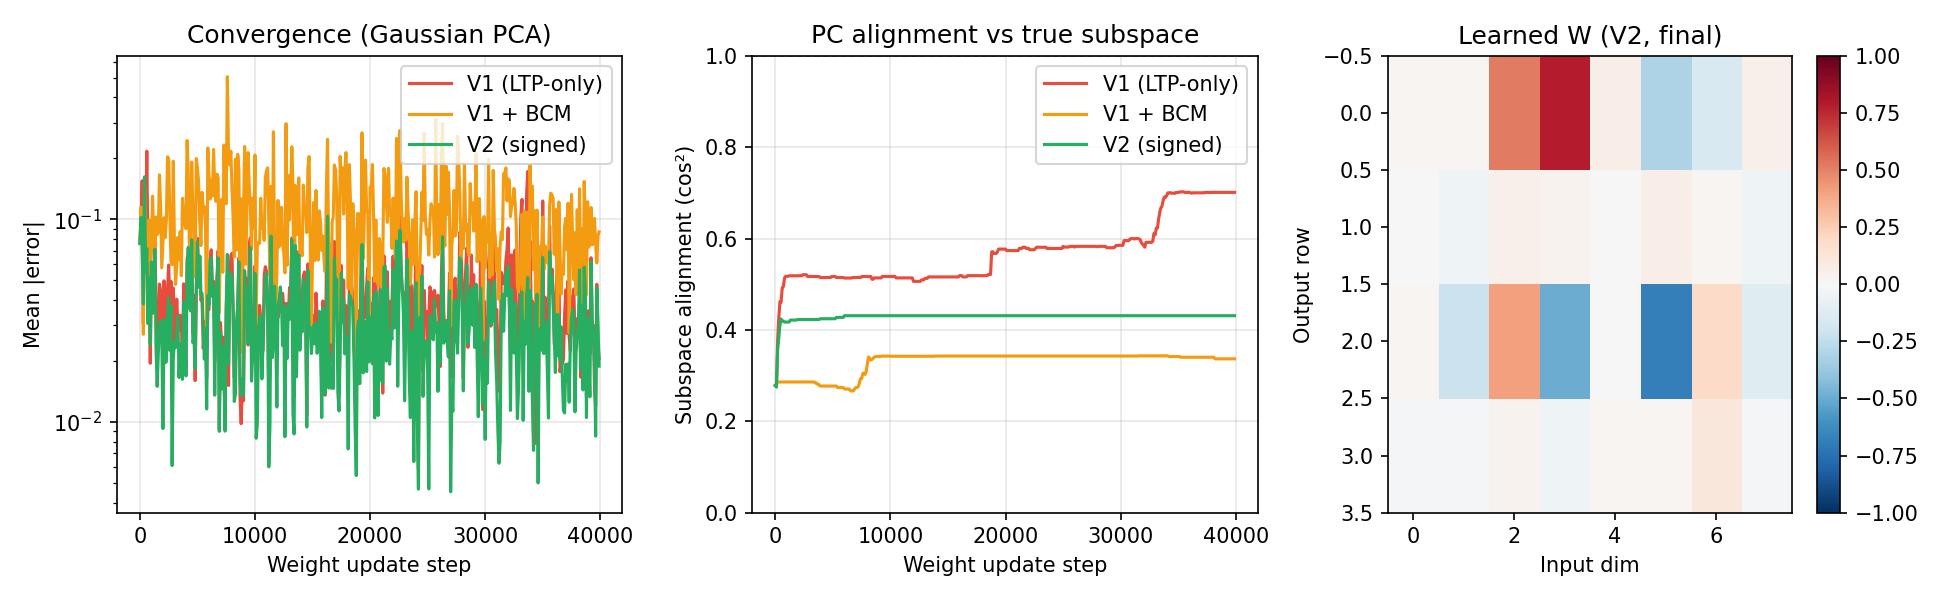
\includegraphics[width=\columnwidth]{../sim/results/e1_gaussian_pca.png}
\caption{E1: Mode comparison on a Gaussian PCA task
($n_\text{in}=8$, $n_\text{rows}=4$, SNR~=~20\,dB, 8 epochs).
V1 (LTP-only) achieves 0.70 subspace alignment and
converges to a gate-quiescent fixed point;
V2 (signed, four-quadrant) reaches 0.43 alignment.}
\label{fig:e1}
\end{figure}

V1 (LTP-only) achieves final subspace alignment 0.70 and prediction error
0.021, converging to a gate-quiescent state.
V2 (signed) achieves 0.43 alignment; discrete weight steps introduce
oscillations near the fixed point when equal-magnitude LTP and LTD updates
compete.
V2 with competitive 2-winner-take-all gating achieves 1.00 template
selectivity on a 16-dimensional dictionary-learning task.
8-bit weight quantisation reduces reconstruction MSE from 0.018 to 0.287
but preserves subspace alignment (0.41 vs.\ 0.43 float), confirming that
6.6-effective-bit weight resolution does not prevent principal subspace
extraction.

\subsection{Temporal Reuse Convergence}

\begin{figure}[t]
\centering
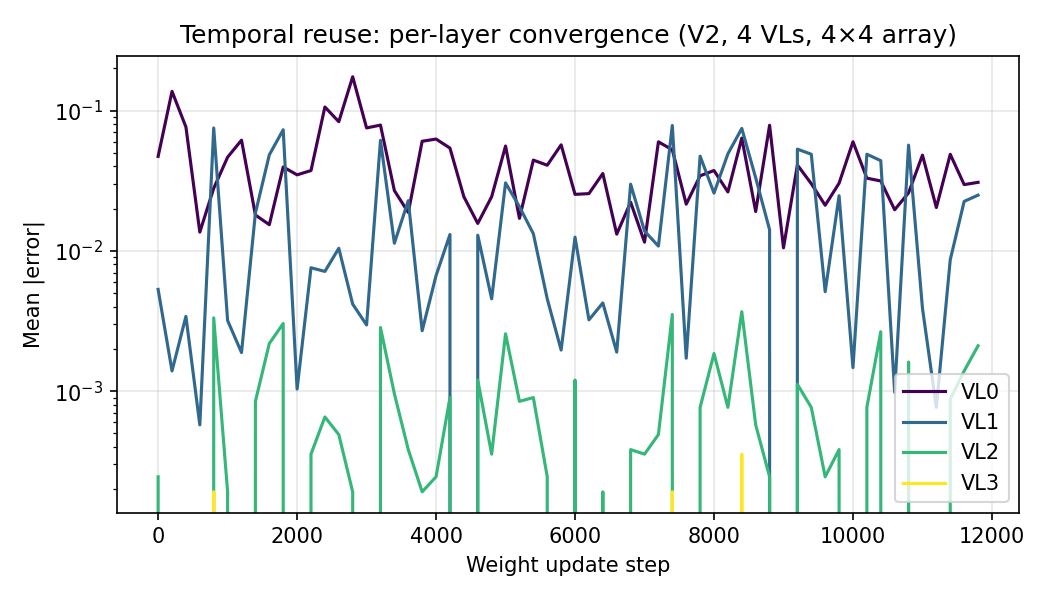
\includegraphics[width=\columnwidth]{../sim/results/e4_temporal_reuse.png}
\caption{E4: Temporal reuse convergence (4-virtual-layer stack,
$4\times4$ array, V2 mode, 3 epochs $\times$ 4{,}000 samples).
Per-layer prediction errors decrease monotonically:
VL0\,=\,0.031, VL1\,=\,0.025, VL2\,=\,0.002, VL3\,$\approx$\,0.}
\label{fig:e4}
\end{figure}

All four virtual layers converge; deeper layers receive progressively more
residualised input and reach lower final error.
$V_\text{inp,cm}$ remains within $\pm 25\,\text{mV}$ of $V_\text{cm}$
across all layers, confirming the operating-point reset.

\subsection{Multi-Cell Predictive Network Validation}
\label{sec:predictive_network}

\begin{figure}[t]
\centering
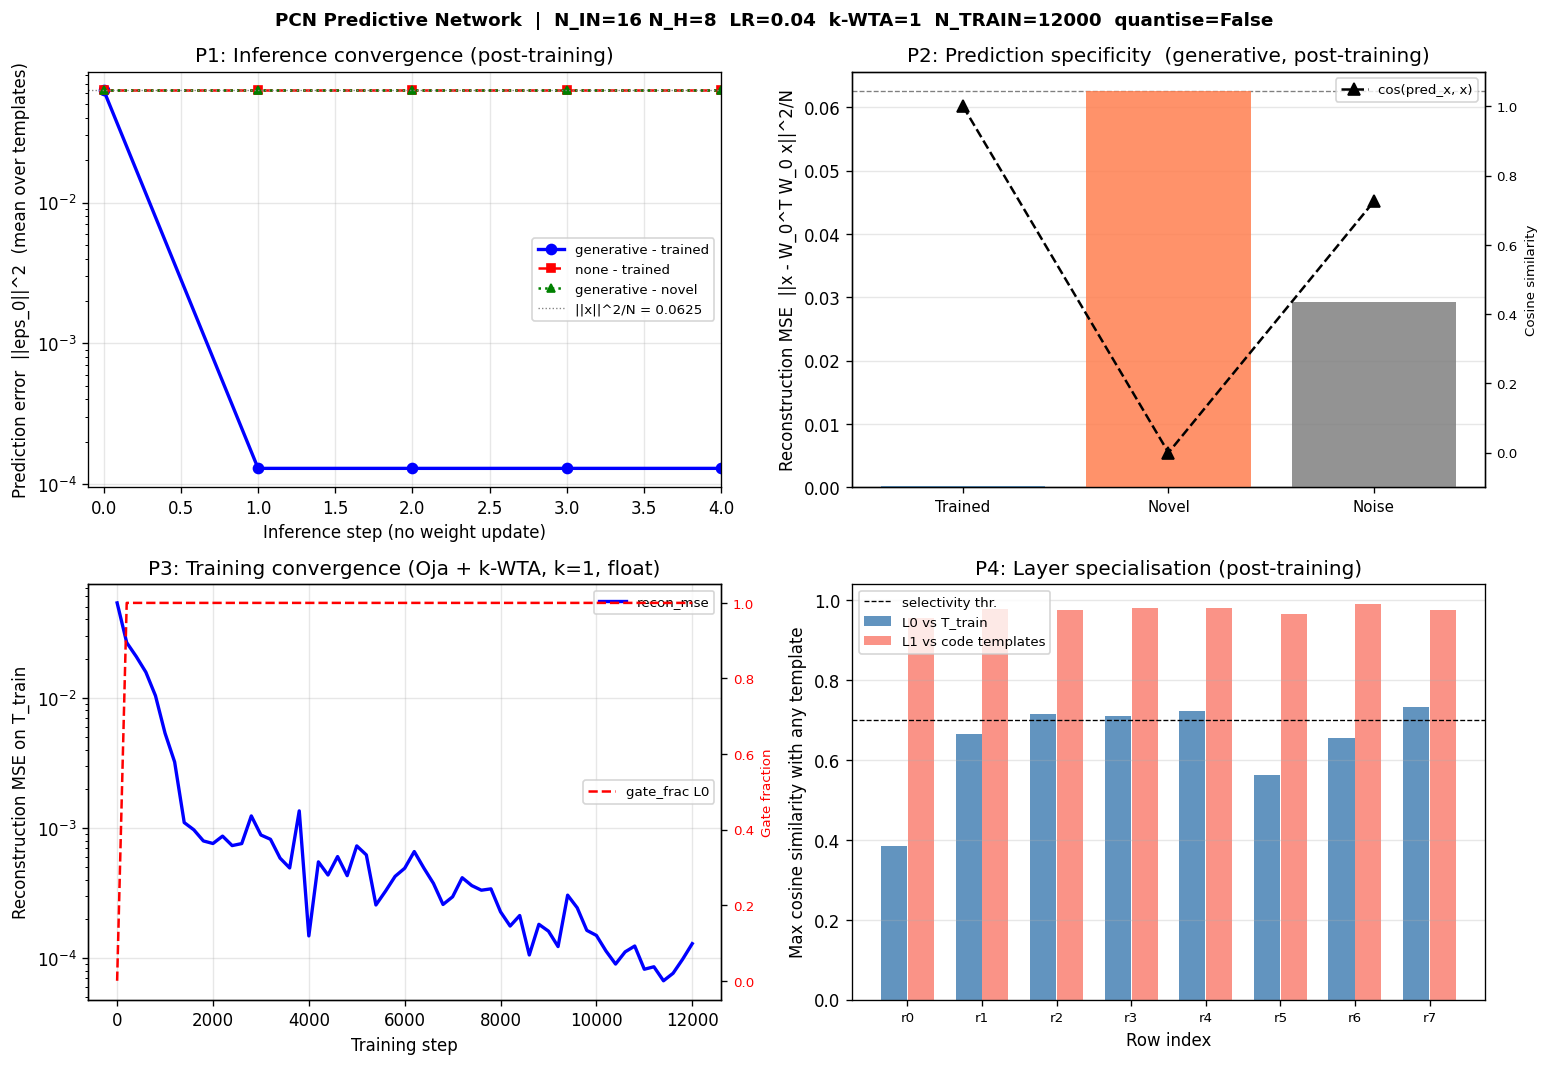
\includegraphics[width=\columnwidth]{../sim/results/p_predictive_network.png}
\caption{Multi-cell predictive network
($N_\text{in}=16$, $N_H=8$, GHA + cosine-decaying LR, 12{,}000 steps).
P1: single-step inference error ratio 484$\times$.
P2: trained MSE $483\times$ below novel.
P3: training convergence.
P4: Layer-1 100\% row selectivity in code space.}
\label{fig:predict}
\end{figure}

A two-layer undercomplete PCN ($\mathbf{W}_0$: $8\times16$,
$\mathbf{W}_1$: $8\times8$) is trained with GHA on Layer~0
and $k=1$ WTA Oja on Layer~1.
Eight orthonormal templates and eight orthogonal novel templates are
generated by QR decomposition.

\textbf{Results.}
After training, a single generative inference step reduces prediction error
from $0.0625 = \|\mathbf{x}\|^2/N$ to $1.3\times10^{-4}$
— a $\mathbf{484\times}$ reduction.
Novel templates maintain prediction error 0.0625 at all inference steps:
the network makes no prediction for inputs it has not seen.
Trained-template MSE $= 1.3\times10^{-4}$ vs.\ novel MSE $= 0.0625$ gives
$\mathbf{483\times}$ specificity.
Layer~1: 100\% row selectivity (cos~$>$~0.7); Layer~0: 99.8\%
subspace coverage.

\textbf{Correct training rule.}
Three simulation failures during development identified the correct rule.
(i)~Without deflation, all rows converge to the same principal direction.
(ii)~$k$-WTA alone creates dead neurons: rows receiving negative Oja updates
cannot recover.
(iii)~Chaining $\mathbf{W}_1^\top\mathbf{W}_1$ in the prediction path
amplifies by up to $N_H\times$, causing inference divergence.
The correct architecture uses GHA on Layer~0 (guaranteed orthonormal
convergence), excludes Layer~1 from the prediction path
($\hat{\mathbf{x}} = \mathbf{W}_0^\top\mathbf{W}_0\mathbf{x}$,
a bounded projector), and applies $k$-WTA only to Layer~1.
All six quantitative checks pass.

\subsection{Real-World Classification Benchmarks}

As a further hardware-faithful validation, Python simulations of the full
GHA pipeline were applied to standard image classification benchmarks:
83.3\% test accuracy on MNIST (10-class digit recognition, 60{,}000 training
samples) and 64.0\% on EMNIST-Letters (26-class, 124{,}800 training samples),
both using only a logistic regression head on the analog-faithful
(8-bit quantised, ReLU-clamped) GHA features — confirming that the
learned representations capture discriminative structure in real-world data.

%% ─────────────────────────────────────────────────────────────────────────────
\section{Discussion}
\label{sec:discussion}

\subsection{Five-Transistor Topology and Its Consequences}

The five-transistor OTA couples tail current to weight voltage and input
common-mode through MN3.
This causes gain variation across spatial layers in the untrained state
(mod0~$= 1.43$, mod1--3~$= 0.45$--$0.70\,\text{V/V}$) and couples power
draw directly to weight encoding.
Both are self-corrected by Hebbian learning; temporal reuse additionally
eliminates cascade-depth drift by resetting $V_\text{cm}$ at each virtual
layer.
A Gilbert-cell topology~\cite{gilbert1968precise} with independent tail
biasing would eliminate both couplings structurally in a next-generation cell.

\subsection{Practical Scope of the Proof-of-Concept}

The Sky130A chip implements one virtual tile: a single 16$\times$16
physical array cycling through up to 8 virtual layers with SRAM-backed
weight persistence, Hebbian learning, and a Wishbone CPU interface.
It is functionally complete as a feature extractor or first-layer encoder.
A full autonomous PCN additionally requires the upward transpose product
$\mathbf{W}^\top\boldsymbol{\varepsilon}$ for representation update,
which would require a second MAC array or time-multiplexed transpose
access — a substantial extension left for future work.

\subsection{Dynamic Routing: Simulation Status}

The routing Hebbian write mechanism is verified in SPICE
(Section~\ref{sec:routing}).
End-to-end convergence of routing weights to a functionally correct learned
topology requires a testbench that simultaneously trains MAC weights and
routing weights over many inference cycles.
The theoretical basis — routing weights as Hebbian MAC weights at a different
hierarchical level — is well-founded on the existing simulation evidence,
but experimental demonstration is deferred to future work.

\subsection{Comparison to Prior Neuromorphic Hardware}

\begin{table}[t]
\caption{Comparison to prior neuromorphic hardware}
\label{tab:prior_work}
\centering
\footnotesize
\resizebox{\columnwidth}{!}{\begin{tabular}{P{1.6cm}P{0.9cm}P{1.4cm}P{1.5cm}P{1.5cm}}
\toprule
Work & Tech & Learning & Capacity & Architecture \\
\midrule
Loihi~2~\cite{davies2018loihi} & 7\,nm & STDP & digital SRAM & spike-based \\
BrainScaleS-2~\cite{pfeiffer2018deep} & 65\,nm & backprop & 64\,syn/mm$^2$ & mixed-signal \\
DynapSEL~\cite{chicca2014neuromorphic} & 180\,nm & STDP & $\sim$40\,syn/mm$^2$ & current-mode \\
Oh~\cite{oh2026synthesizable} & Digital RTL & Supervised PC & SRAM weights & seq.\ MAC+FSM \\
\textbf{This work} & 130\,nm & Hebbian PCN & $256\times N_v$/cell & temporal + routing \\
\bottomrule
\end{tabular}}
\end{table}

The structural differences from prior work are:
(i) rate-coded rather than spike-coded learning, enabling continuous
activations and the PCN hierarchical generative model;
(ii) temporal multiplexing, decoupling weight capacity from analog area;
(iii) dynamic routing at the inter-module level;
(iv) zero off-chip weight bandwidth at inference, regardless of effective
network depth.

\subsection{Claims, Evidence, and Open Questions}
\label{sec:validation}

The evidence base spans three levels, and distinguishing them is important
for assessing the work's current standing.

\textbf{SPICE-verified (circuit level).}
Seven circuit checks (Table~\ref{tab:circuit}) validate individual block
behaviour against analytical predictions using Sky130A PDK models.
The PMOS source-follower level shift ($+0.67$\,V), spatial cascade gains
(mod0--3), and temporal reuse gain (6.68\,V/V) are direct SPICE measurements.
All results are reproducible from the published netlist.

\textbf{Tool-verified (digital synthesis and P\&R).}
1,117 standard cells, $+8.46$\,ns setup margin, zero routing DRC violations.
These are tool outputs, independent of simulation assumptions, and
reproducible from the published RTL.

\textbf{Software-verified (algorithmic simulation).}
484$\times$ prediction error reduction and 483$\times$ specificity are
outputs of open-source Python code on a hardware-calibrated model.
These results are established on synthetic Gaussian tasks;
generalisation to practical data distributions is an open question
that hardware validation will address.

\textbf{Pre-silicon projections (estimated).}
All absolute power figures, node-scaling projections (Tables~\ref{tab:node_scaling},
\ref{tab:multichip}), TOPS/W comparisons, and NVM technology projections
in Section~\ref{sec:cw_scaling} are engineering estimates from
standard scaling rules and published literature values.
They have not been validated by analog simulation at smaller geometries.
The energy comparison (Table~\ref{tab:gpu_comparison}) correctly reflects
the memory-bandwidth argument but compares architecturally different systems
at different numerical precision and task scope; it is not a
task-equivalent benchmark.

\textbf{Path to silicon validation.}
Tape-out via Efabless OpenMPW is targeted as the primary validation step.
The critical experiment is end-to-end multi-cell operation: a full
16$\times$16 array with SRAM-backed temporal reuse and live Hebbian updates,
measured in silicon against the SPICE-calibrated software predictions.
All design files, RTL, and simulation scripts are open-source at
\url{https://github.com/dobneyresearch/PredictiveCodingNetworks_AnalogVLSIdesign},
enabling independent verification of every circuit and algorithmic claim
prior to fabrication.

%% ─────────────────────────────────────────────────────────────────────────────
\section{Conclusion}
\label{sec:conclusion}

We have presented an analog VLSI architecture for Predictive Coding Networks
that addresses the three key barriers to scalable analog neural computation:
weight density (via temporal layer reuse), fixed topology (via learned
routing weights), and quiescent power (via precision-gate co-scaling).

The Sky130A proof-of-concept is fully verified at the simulation level:
SPICE-validated analog blocks, a 22-state digital controller synthesised in
1,117 standard cells, place-and-route closed at $+8.46$\,ns setup margin
with zero routing DRC violations.
Software simulation with the hardware-calibrated model achieves
484$\times$ single-step prediction error reduction and 483$\times$
specificity with GHA-trained weights, and identifies the correct training
rule and three hardware design rules from simulation failures.

The architecture scales naturally along two orthogonal dimensions.
Temporal reuse decouples effective weight capacity from analog area;
dynamic routing allows the network to discover inter-chip prediction
topology from data.
Multi-chip systems scale linearly — chips are independent, the inter-chip
interface is 8-bit digital SPI, and no synchronisation overhead arises
as the system grows.

A second and independent scaling dimension is area rather than geometry.
The PCN's locally connected Hebbian update requires no cross-chip gradient
synchronisation, so parameter capacity grows linearly with silicon area
at a fixed node.
At 28\,nm — the last geometry with continuous transistor width sizing and
adequate VDD headroom for the 5T OTA — a 25\,mm$^2$ die holds
$\approx$59\,M effective weights at $\approx$50\,mW.
At wafer scale, the same tile pattern yields $\approx$460 billion effective
weights at $\approx$114\,W.
The locality of Hebbian learning eliminates the global gradient-bus
complexity that constrains backprop-based wafer-scale designs, positioning
the PCN as a candidate architecture for large-scale analog learning systems
where the scaling bottleneck is area rather than geometry.

All performance claims are pre-silicon simulation results; the Sky130A
tape-out will provide the first silicon-validated evidence for the
operating-point, gain, power, and learning dynamics described here.

%% ─────────────────────────────────────────────────────────────────────────────
\section*{Acknowledgements}

The author used Anthropic Claude Code~\cite{anthropic2025claudecode} for
assistance with circuit design, RTL development, Python simulation, and
manuscript preparation throughout this work.

%% ─────────────────────────────────────────────────────────────────────────────
\bibliographystyle{IEEEtran}
\bibliography{refs}

\end{document}
